\documentclass{article}
\usepackage[T2A]{fontenc}
\usepackage[utf8]{inputenc}

%Hyphenation rules
%--------------------------------------
\usepackage{hyphenat}
\hyphenation{ма-те-ма-ти-ка вос-ста-нав-ли-вать ра-дио-тех-ни-чес-ких}
%--------------------------------------

\usepackage{amsmath,amssymb}
\usepackage[russian,english]{babel}
\usepackage{subfigure}

\renewcommand\thesubfigure{\asbuk{subfigure}}

\usepackage{graphicx} %package to manage images
\graphicspath{{./images/}}

\usepackage[a4paper,
bindingoffset=0.2in,
left=1in,
right=1in,
top=1in,
bottom=1in,
footskip=.25in]{geometry}

%\renewcommand\figureshortname{Рис.}

\title{\begin{otherlanguage*}{russian}
		\textbf{Решение задачи сверхразрешения с использованием полносвязной модели нейронной сети}
\end{otherlanguage*}}

% переименовываем  список литературы в "список используемой литературы"
\addto\captionsrussian{\def\refname{Список используемой литературы}}



\begin{document}
	
	\maketitle
	
	\section*{Аннотация}
	В работе приведена математическая модель цифровой антенной решетки (ЦАР) для определения положения объектов в угломерном пространстве. Поставлена задача определения положения нескольких объектов с ЦАР различной конфигурации. Сформулирована задача определения значений коэффициентов принятого сигнала на приемных устройствах решетки, позволяющая решать задачу сверхразрешения на основе задачи экстраполяции. Приведен метод решения задачи экстраполяции на основе модели полносвязной нейронной сети прямого распространения. Описаны практические результаты решения задачи сверхразрешения как с выбранной моделью, так и в сравнении с другим методом экстраполяции.
	
	\section*{Введение}
	Повышение информативности угломерных систем является актуальной научной и технической проблемой. Поисковые задач, связанные с определением положения или очертанием границ объектов, нахдодят большое приложения в таких различных областях науки как сейсмика, геология, акустика, электромагнетизм и т.д. Улучшение точности угловых измерений и эффективной угловой разрешающей способности с использованием новых методов цифровой обработки сигналов является важным шагом в направлении развития таких информационных радиотехнических систем.
		
	Радиолокационные системы (РЛС), основанные на цифровых антенных решетках (ЦАР), преобразуют сигналы в цифровую форму и обрабатывают их с помощью специальных алгоритмов. ЦАР способны анализировать и обрабатывать гораздо больше информации, содержащейся в структуре принимаемого сигнала, чем обычные антенны. В результате возможно достижение разрешающей способности, превышающей предел, определенный критерием Рэлея - сверхразрешение.
	
	Методы обработки принятого сигнала на основе ЦАР подходят для широкого класса задач, основанных на волновых процессах, где необходимо исследовать положение объектов и границ, например в задачах гидролокации, сейсмических исследованиях, акустике. Приведенные задачи относятся к классу поисковых, в которых важен как результат различия разных объектов так и точность их поиска, что увеличивают значимость данного исследования.
	
	Угловое разрешение, основанное на критерии Рэлея, может быть выражено следующим образом:
	
	\begin{equation} \label{raileigh}
			\delta \theta \approx \lambda\ /\ D
	\end{equation}
	
	где $D$ - линейный размер антенны, $\lambda$ - длина волны, которая соответствует ширине диаграммы направленности (ДН) до половинной мощности.
	
	Из-за важности задачи повышения углового разрешения во многих странах разрабатываются и внедряются методы цифровой обработки сигналов, которые позволяют превысить (1) и достигать сверхразрешения. \cite{lit1, lit2, lit3, lit4, lit5, lit6}
	
	\section*{Постановка задачи}
	
	Принятый со стороны ЦАР сигнал $U(\alpha)$ может быть модельно представлен в виде интегрального преобразования:
	
	\begin{equation} \label{U_alpha}
		U(\alpha) = \int \limits_{\Omega}^{} F(\alpha - \varphi) I(\varphi) d\varphi,
	\end{equation}
	где $\Omega(\alpha)$ - угловая область (сектор сканирования) расположения источника сигнала; $I(\alpha)$ - угловое распределение амплитуды отраженного (или излучаемого сигнала), равное $0$ вне $\Omega$; $F(\alpha)$ - ДН измерительной системы. Достигаемая при проведении прямых измерений в соответствии с (\ref{U_alpha}) угловая разрешающая способность совпадает с классической величиной (\ref{raileigh}).
	
	Для ЦАР ставится задача на основе интеллектуального анализа принятого сигнала $U(\alpha)$ и известной ДН системы $F(\alpha)$ восстановить изображение источника сигналов $I(\alpha)$ с угловым разрешением, превышающим критерий Рэлея, во много более возможном масштабе.
	
	В математическом аспекте задача сводится к приближенному решению (\ref{U_alpha}), рассматривамому как линейное интегральное уравнение (ЛИУ) Фредгольма первого рода типа свёртки относительно неизвестной функции $I(\alpha)$, с максимально достижимой точностью.
	
	В общем случае попытки увеличить разрешение по сравнению с (\ref{raileigh}) путём решения ЛИУ (\ref{U_alpha}) приводят к появлению неустойчивых решений, т.к. поставленная задача относится к классу обратных и не удовлетворяет второму и третьему требованию корректности задачи по Адамару \cite{lit3, lit7, lit8, lit9, lit10}.
	
	\section*{Метод решения}
	
	Для ЦАР возможен иной подход к задаче, напрямую не сводящийся к решению ЛИУ (\ref{U_alpha}), что повышает устойчивость используемых алгоритмов.
	
	Для упрощения получаемых выражений рассмотрим большую линейную ЦАР с числом элементов $2N + 1$. Амплитуды токов на излучателях полагаем равными, область расположения источника $\Omega$ - одномерной, с размерами меньшими ширины луча ЦАР $\theta_{0.5}$. Значения амплитудных ДН отдельных излучателей ЦАР в пределах $\theta_{0.5}$ считаем не изменяющимися. Тогда, заменив $sin(\alpha) \approx \alpha$, ДН решётки можно представить в виде:
	
	\begin{equation} \label{DN}
	F(\varphi - \alpha) = \sum\limits_{n=-N}^{N} exp(ikdn(\varphi - \alpha))
	\end{equation}
	где $k = 2\pi/\lambda$ - волновое число, $d$ - расстояние между соседними излучателями, $\alpha$ - направление максимума ДН. Для ЦАР сигнал (\ref{U_alpha}) при введённых условиях преобразуется в сумму:
	
	\begin{equation} \label{general_U}
	U(\alpha) = \sum_{n=-N}^{N}exp(-ikdn\alpha)\int\limits_{\Omega}^{}exp(ikdn\varphi)I(\varphi)d\varphi=\sum\limits_{n=-N}^{N}C_n exp(-ikdn\alpha),
	\end{equation}

	\begin{equation} \label{coeffs_Cn}
	C_n = \int\limits_{\Omega}^{} exp(ikdn\varphi)I(\varphi)d\varphi, n = 0, \pm 1, \dots, \pm N, 
	\end{equation}
	где коэффициенты $C_n$ - сигнал, принятый $n$-ым элементом ЦАР.
	
	Обобщение (\ref{general_U}) и (\ref{coeffs_Cn}) и получаемых в дальнейшем выражений на общий случай, в том числе и на двумерные задачи, принципиальных трудностей не вызывает.
	
	Ядро ЛИУ (\ref{U_alpha}) для ДН в виде (\ref{DN}) является вырожденным. Несложно показать, что в этом случае решение $I(\alpha)$ выражается посредством коэффициентов $C_n$:
	\begin{equation} \label{kernel}
			I(\alpha) = A\sum_{n=-N}^{N} exp(-ikdn\alpha)C_n + \psi(\alpha)
	\end{equation}
	где $\psi(\alpha)$ - произвольная функция, ортогональная всем собственным функциям ядра, т.е. экспонентам из (\ref{kernel}) на отрезке $[-\lambda/d;\lambda/d]$, $A$ - нормировочный коэффициент.
	
	Конкретный вид функции $psi(\alpha)$ не может быть непосредственно найден из условий задачи. Для её определения или хотя бы оценки требуется какая-либо априорная информация. Приближенное решение, которое представлено первым слагаемым суммы (\ref{kernel}), повторяет по форме сигнал $U(\alpha)$, и следовательно, полученное разрешение соотвествует критерию Рэлея.
	
	Рассмотрим одну из возможностей увеличения углового разрешения ЦАР. В отличие от обычных фазированных антенных решеток (ФАР), сигналы, принятые каждым излучателем ЦАР - $C_n$, могут быть зарегистрированы в цифровом виде и применены далее при цифровой обработке.
	
	Из (\ref{coeffs_Cn}) следует, что различия значений $C_n,\ n = 1, 2, \dots$ определяются только пространственным положением отдельных излучателей ЦАР. Следовательно, проанализировав расположение достаточно большого количества излучателей и значения соотвествующего им набора коэффициентов $C_n$, можно с определенной точностью найти зависимость принимаемого сигнала $C_j$ от координат или положения излучателя на решетке, что позволит с определенной точностью оценить значения принимаемого сигнала виртуальными излучателями за пределеами апертуры ЦАР и, с определенной точностью, продолжить эту зависимость. Далее, используя прогнозные значения $C_j, \ j = \pm (N+1), \pm (N+2), \dots, \pm M$ вместе с измеренными ранее значениями $C_j, j = -N, -N + 1, \dots, N$, распространим суммирование в (\ref{general_U}) до $2M + 1$ членов.
	В результате получим ДН виртуальной ЦАР с $2M + 1$ излучателями и увеличенной в $M/N$ раз апертурой. Ширина ДН уменьшилась во столько же раз, и при идеальных условиях, в $M/N$ раз увеличиваются точность угловых измерений и угловая разрешающая способность.
	
	В итоге, восстановленное со сверхразрешением приближенное изображение объекта представлено в виде:
	
	\begin{equation} \label{extrap_Cn}
		I(\alpha) \approx \sum_{n = - M}^{M} exp(-ikdn\alpha)C_n
	\end{equation}
	где $M$ - количество приемных устройств виртуальной ЦАР в одну сторону от её центра.
	
	Чем больше синтезированная апертура ЦАР, т.е. чем уже ДН, тем, в соответствии с (\ref{raileigh}), выше угловое точное решение и точнее найденное приближенное решение (\ref{extrap_Cn}). В пределе при $N \to \infty$ найдем точное решение, полученное с помощью ДН в виде дельта-функции, которое представляет собой разложение $I(\alpha)$ в ряд Фурье на соответсвующем интервале.
	
	Таким образом, приближённое решение ЛИУ (\ref{U_alpha}-\ref{general_U}) сведено к определению с значений возможно большего количества комплексных коэффициентов C за пределами апертуры ЦАР. Восстановление значений коэффициентов C для виртуальных элементов ЦАР (т.е. за пределами реальной апертуры) может быть выполнено методами экстраполяции.
	
	Для примера задачи обнаружения двух равноинтенсивных объектов gредставим распределение интенсивности источников излучения $I(\alpha),\ \alpha \subset \Omega$ в виде комбинации дельта-функций Дирака \cite{lit22}:
	
	\begin{equation}
		I(\alpha) = \delta(\alpha - t_1) + \delta(\alpha - t_2), \ t_1,t_2 \in \Omega,
	\end{equation}
	где $t_1, t_2$ - известные положения объектов в угловом одномерном пространстве $\Omega$.
	Изобразим возможную зависимость коэффициентов принятого сигнала на приемных устройствах в зависимости от его возможного положения в апертуре ЦАР с равноудаленными приемными устройствами (рис.\ref{fig:1}а).
	 
		\begin{figure}[h]
		\centering
		\subfigure[]{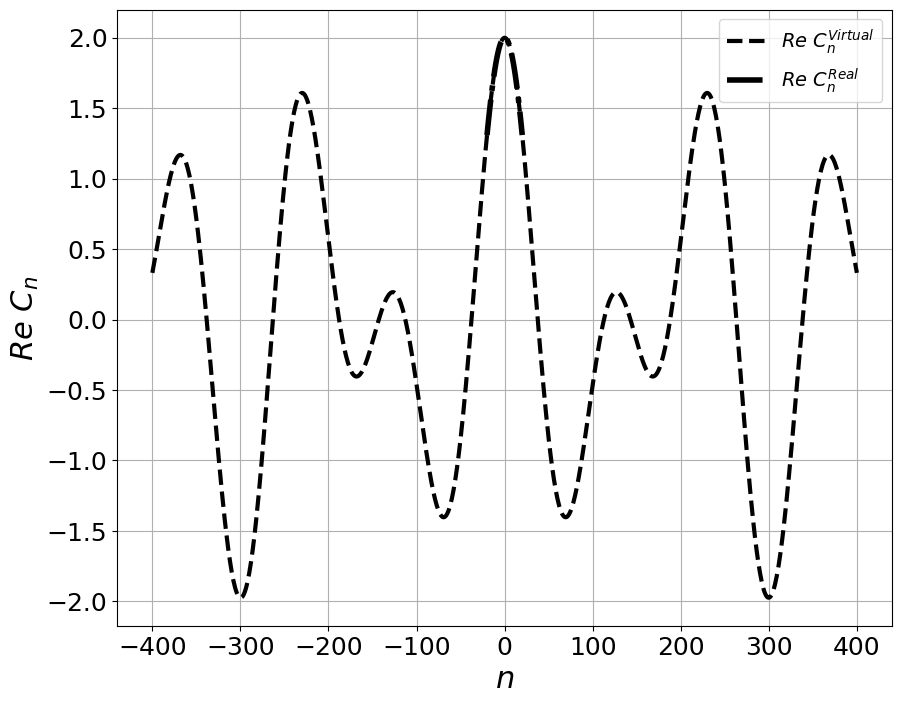
\includegraphics[width=0.45\textwidth]{Begin_virtual_bw.png}}
		\subfigure[]{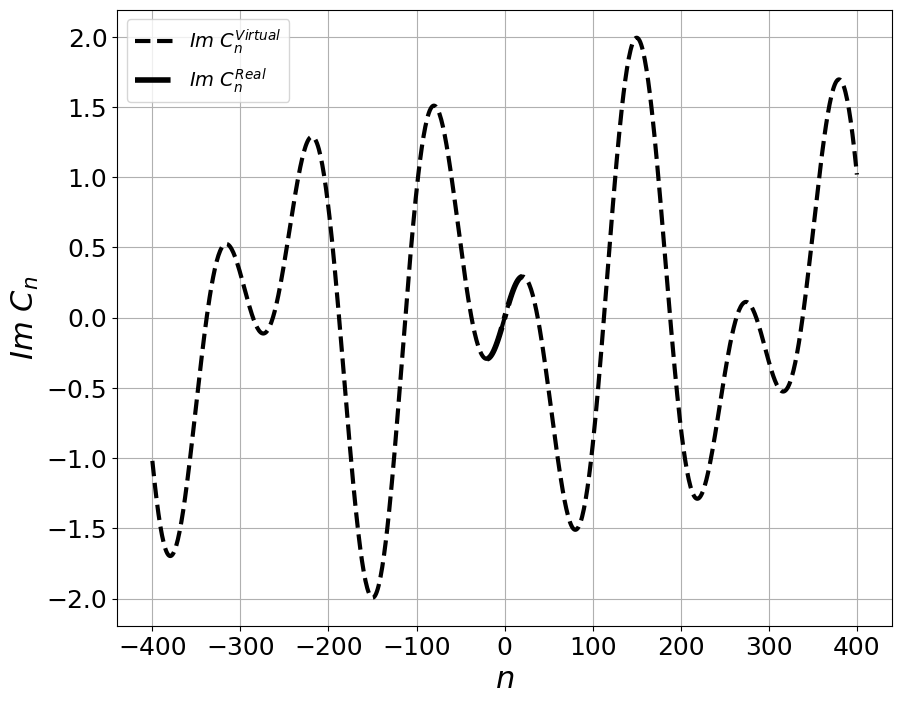
\includegraphics[width=0.45\textwidth]{Begin_virtual_imag_bw.png}}
			\caption{(а) действительная часть комплексных значений принятого сигнала на приемных устройствах в зависимости от номера позиции в ЦАР, (б) Мнимая часть комплексных значений принятого сигнала на приемных устройствах в зависимости от номера позиции в ЦАР; сплошная жирная линия - значения на физических устройтвах ЦАР в соответствии с выражением (\ref{coeffs_Cn}); штриховая линия - значения на возможных виртуальных устройствах ЦАР в соответствии с выражением (\ref{coeffs_Cn}) в предположении о возможном расширении физической конфигурации ЦАР}
		\label{fig:1}
		\end{figure}
	
	На рисунке выше (рис.\ref{fig:1}а) можно предположить что теоретическая функция действительных значений принятого сигнала в зависимости от номера устрйоства является четной, то есть симметричной относительно $n=0$. Экстраполяция действительных значений необходима лишь в одну сторону с зеркальным отображением возможных предсказанных значений в другую относительно центрального устройства. Заметим также что модельная теоретическая зависимость несимметричных целей является осциллирующей как комбинация нескольких гармонических составляющих, а также затухающей по амплитуде значений, что показывает возможную сложность в экстраполяции значений на основе классических интегральных кривых решения динамических систем.
	
	Также приведем иллюстрацию зависимости мнимых частей значений принятого сигнала на физических и модельных виртуальных устройствах ЦАР (рис.\ref{fig:1}б) в случае, если объекты расположены несимметрично относительно центра области наблюдения $|t_1| \ne |t_2|$, то есть объекты неравноудалены от начала координат.
		
	На рисунке (рис. \ref{fig:1}б) заметим, что теоретическая модельная зависимость возможных мнимых значений принятого сигнала на виртуальных устройствах при конкретной реализации объектов в угломерном пространстве представлена в виде нечетной функции, то есть в виде функции сопряженных значений относительно центра ЦАР $n = 0$. Из графиков зависимостей (рис\ref{fig:1}) можно сделать вывод о достаточности решения задачи экстраполяции комплексных значений принятого сигнала на устройствах ЦАР при заданных $K$ физических устройствах только в одну сторону от центра ЦАР, то есть в положительную полуось положений виртуальных устройств и значения в отрицательной полуоси представлять сопряженными к полученным значениям.
	
	В результате решения задачи экстраполяции на основе полученных оценок $\hat{C}_n,\ n\in [-M, M]$ возможно восстановить распределение принятого сигнала $U(\alpha)$ на ЦАР так, как если бы в сканировании области с интенсивностью $I(\alpha)$ принимало участие $2\cdot M + 1$ устройств. По итогам мы имеем возможность получить изображение объектов с большим разрешением, превышающим критерий Рэлея для физической ЦАР заданной конфигурации (рис.\ref{fig:2}).
	
		\begin{figure}[h]
		\centering
		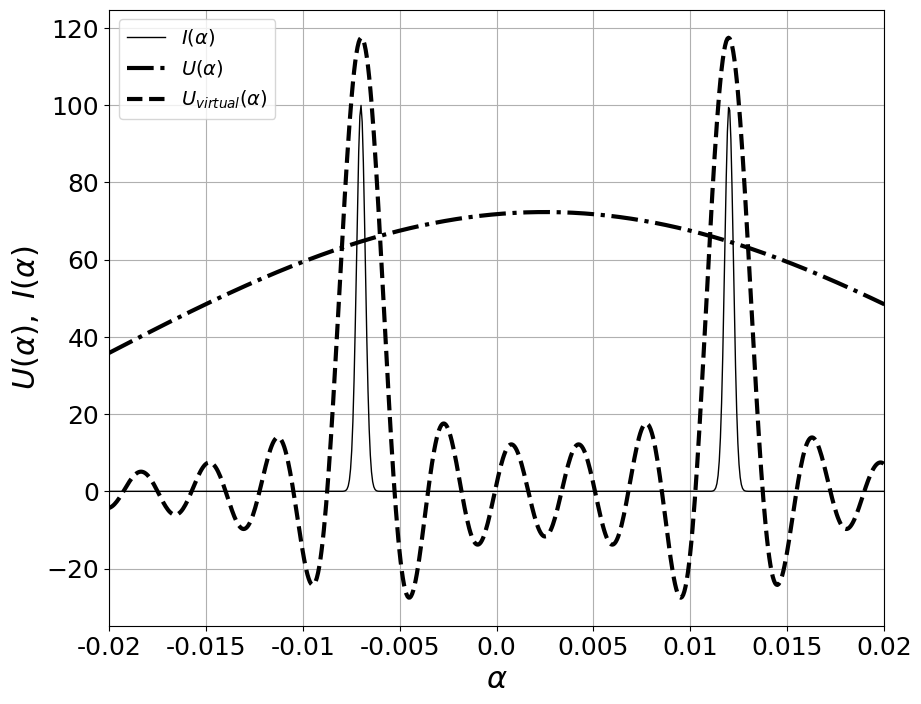
\includegraphics[width=0.65\textwidth]{Begin_target_bw.png}
		\caption{Значения функции распределения интенсивности источников и распределение принятого сигнала на ЦАР в угловом пространстве $\alpha \subset \Omega$; сплошная тонкая линия - значения распределения интенсивности объектов $I(\alpha)$, моделируемых на основе дельта-функций Дирака \cite{lit22}; штриховая жирная линия - принятый сигнал на физической ЦАР, рассчитанный на основе (\ref{general_U}); сплошная жирная линия - принятый сигнал, , рассчитанный на основе (\ref{general_U}), с применением моделируемых виртуальных устройств при их идеальной работе в соответсвтии с моделью (\ref{DN})}
		\label{fig:2}
		\end{figure}
	
	
	
	Существует множество видов экстраполяции (линейные, полиномиальные, сплайновые и~т.~д.), которые характеризуются различными показателями сложности вычислений и быстродействием. В данной работе приводится решение задачи экстраполяции значений принятого сигнала на основе полносвязной модели нейронной сети прямого распространения \cite{lit18}, \cite{lit19}.
	
	Принцип прогнозирования зависимостей на основе алгоритмов искуственных нейронных сетей (ИНС) широко применяется в различных областях науки и техники последние 20 лет. ИНС часто используются в прикладных задачах распознавания образов, детекции объектов на изображениях и видео, генерации и обработки текстовой информации, обработки аудиосигналов, а также в различных прикладных задачах робототехники и управления.
	
	Существует множество разновидностей и архитектур нейронных сетей прямого распространения. Для одномерной задачи, поставленной ранее, мы имеем возможность использовать как полносвязную искусственную нейронную сеть прямого распространения \cite{lit11,lit12,lit13}, так и свёрточные аналоги \cite{lit14,lit15}. Полносвязные нейронные сети прямого распространения применяются в задачах обработки одномерных зависимостей, ввиду простоты архитектуры нейронной сети, скорости работы и эффективности использования вычислений с одномерными зависимостями. По скорости работы и принципу действия в одномерном случае полносвязные и свёрточные нейронные сети идентичны, для ядер свертки размером равным длине входных данных (размерности вектора данных) в сверточных сетях. Для простоты пояснения и построения системы экстраполяции зависимости будем использовать классическую реализацию полносвязной нейронной сети прямого распространения, показав по результатам возможности подобного класса алгоритмов решать поставленную задачу.
	
	Полносвязная нейросетевая модель прямого распространения является функцией, представляемой в виде:

	\begin{equation} \label{FCNN}
		\hat{y} = FCNN(x|W), 
	\end{equation}
	где $W$ - вектор матриц весов (параметров) модели, $x\in \mathbb{R}^{f}$ - вектор значений входного примера, $\hat{y}\in \mathbb{R}^{d}$ - вектор оценки целевых значений. Нейронная сеть отображает вектор входных данных $x$  в выходной вектор оценки $\hat{y}$, посредством серии линейных преобразований с нелинейными функциями активации.
	
	Полносвязная нейросетевая модель состоит из соединенных в скрытые слои линейные нейроны с нелинейной функцией активации. По мере прямого распространения информации от входов к выходу ко входному вектору $x$ применяется последовательная серия линейных преобразований с матрицами весов слоя и нелинейных преобразований на основе выбранных функций активации. Входные данные часто представляются в виде матрицы векторов $X$:	
	\begin{equation}\label{X_input}
		X = (x^{<1>}, x^{<2>}, \dots, x^{<s>}) \in \mathbb{R}^{s \times f}, \ x^{<i>} \in \mathbb{R}^{f},\ i\in 1, 2, \dots, s,
	\end{equation}
	где $s$ - количество примеров, $f$ - размер вектора значений каждого примера.
	Значения на выходе нейронной сети представляются также в виде матрицы оценок $\hat{Y} \in \mathbb{R}^{s\times d}$, где $d$ - размер одного вектора меток, соотвествующий своему входному вектору. 
	
	Каждый слой нейронной сети c $L$ слоями обладает матрицей весов $W^{l},\ l \in 1, 2, \dots, L$, взвешивающей выход из предыдущего слоя или входа на каждом нейроне текущего слоя. Все матрицы весов $W = (W^{1}, W^{2}, \dots, W^{L})$ нейронной сети обладают различными размерами, зависящими от размера входных векторов $f$, требуемого размера выходных векторов $d$ и количества нейронов в каждом из слоев нейронной сети.
	
	Веса нейронной сети $W$ настраиваются в процессе обучения на тренировочной выборке примеров $X_{train}$ и эталонных меток $Y_train$ таким образом, чтобы минимизировать выбранный функционал ошибки $Loss(Y, \hat{Y})$ на пространстве параметров нейронной сети вследствие чего ставится следующая задача оптимизации:
	\begin{equation}\label{opt_problem}
		Loss(Y, FCNN(x|W)) \to \underset{W}{min}
	\end{equation}
	Функционал ошибки между оценками $\hat{Y}$ (\ref{FCNN}) и метками $Y$ выбирается исходя из задачи и должен как отражать качество решения задачи нейронной сетью в виде числовой метрики. Существует множество функционалов качества для различных задач, решаемых алгоритмами искусственного интеллекта \cite{lit24}, \cite{lit25}. Минимизация метрики качества (\ref{opt_problem}) решения задачи (\ref{FCNN}) производится на основе алгоритма из семейства методов градиентного спуска с различными модификациями \cite{lit26} в котором веса $W$ итеративно обновляются на основе тестовых прогонов работы модели на тренировочной выборке $X_{train}$ (\ref{X_input}) и минимизации полученных ошибок между ответами модели (\ref{FCNN}) и метками $Y_{train}$. Качество итогового обучения принято проверять на тестовой отложенной выборке схожих примеров $X_{test}$ в сравнении с эталонными метками $Y_{test}$.
	
	
	\section*{Численные эксперименты и сравнение методов экстраполяции}
	
		\begin{figure}[h]
		\centering
		\subfigure[]{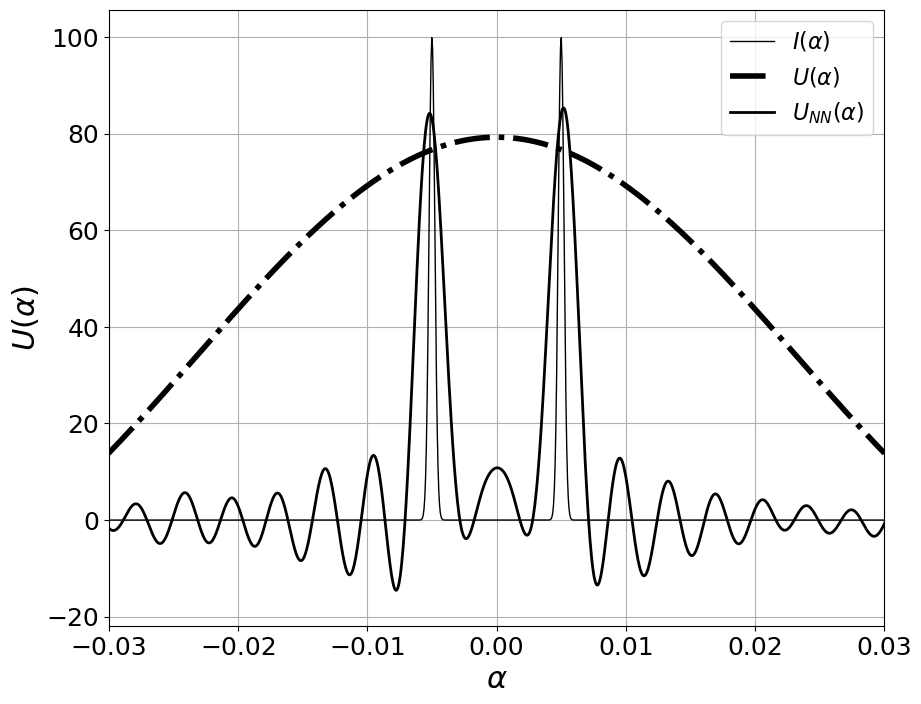
\includegraphics[width=0.45\textwidth]{Complete1_target_bw.png}}
		\subfigure[]{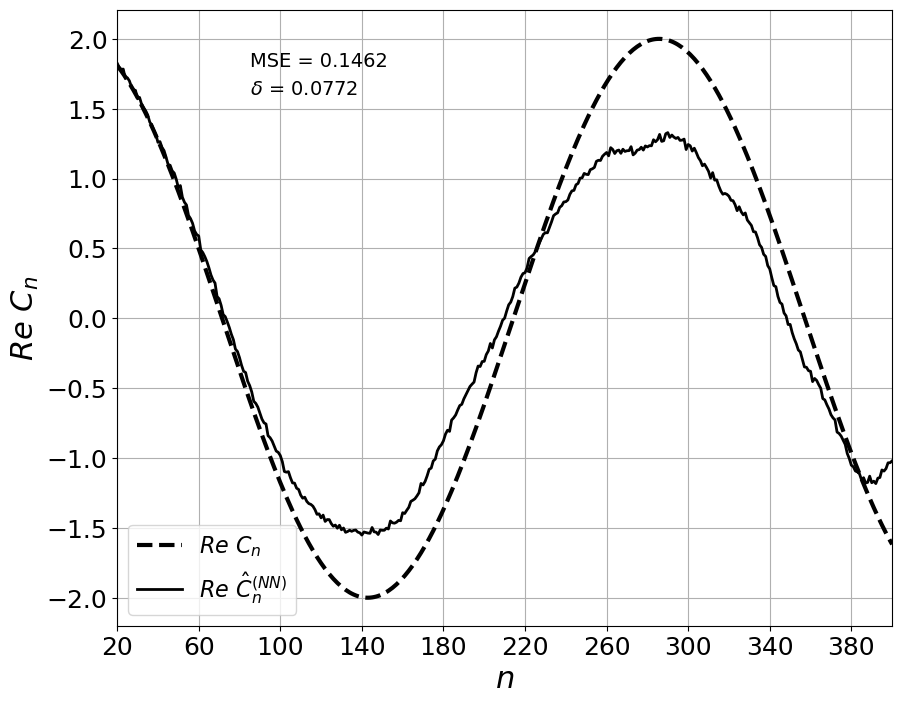
\includegraphics[width=0.45\textwidth]{complete_virtual1_real_bw.png}}
		\caption{}
		\label{fig:3}
	\end{figure}
	
	\begin{figure}[h]
		\centering
		\subfigure[]{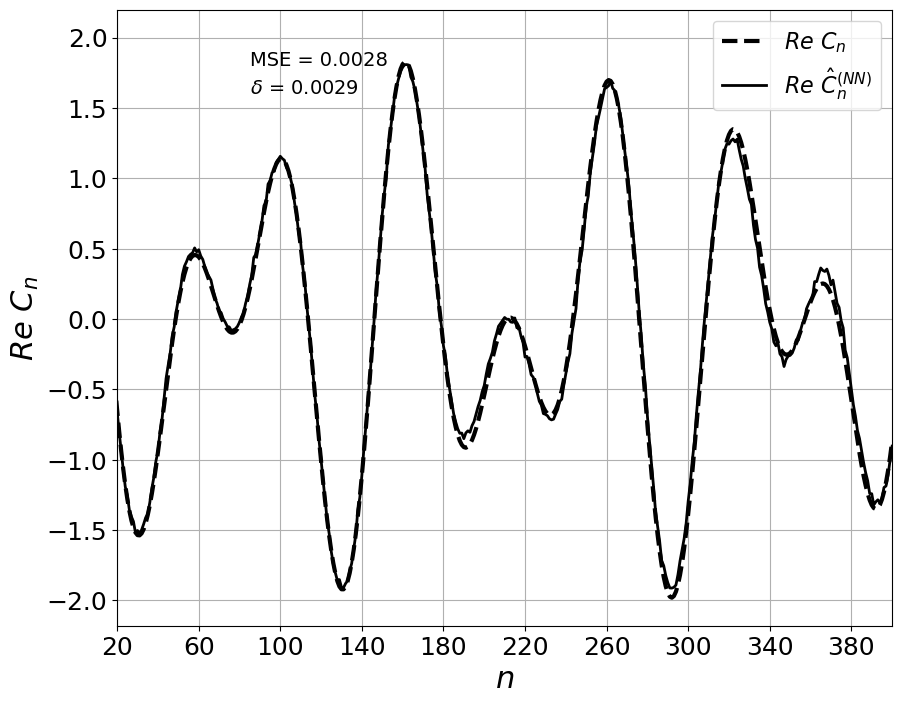
\includegraphics[width=0.45\textwidth]{complete_virtual2_real_bw.png}}
		\subfigure[]{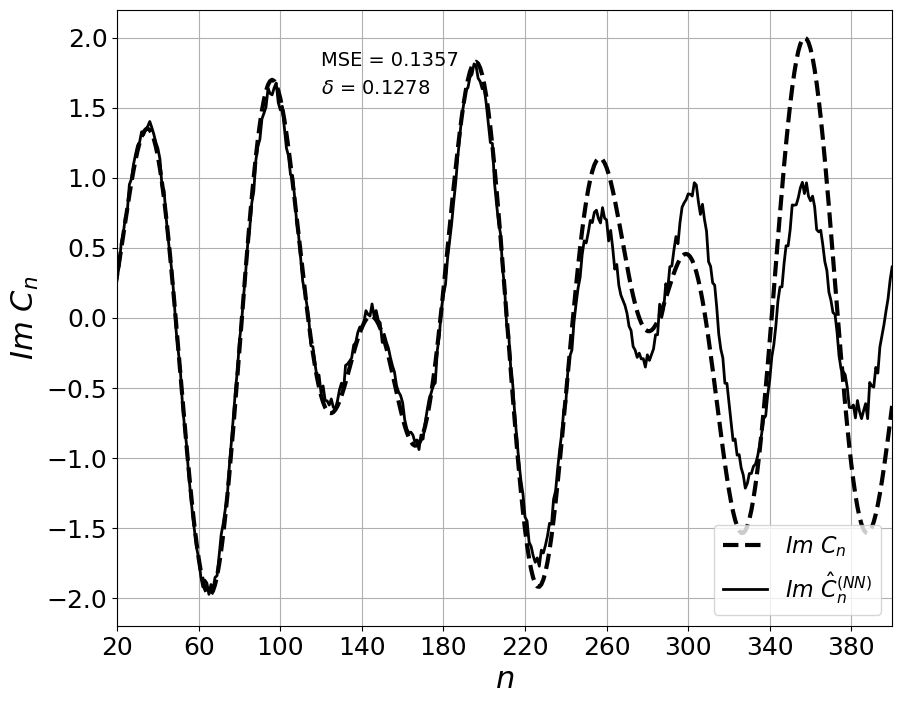
\includegraphics[width=0.45\textwidth]{complete_virtual2_imag_bw.png}}
		\caption{}
		\label{fig:4}
	\end{figure}
	
	\begin{figure}[h]
		\centering
		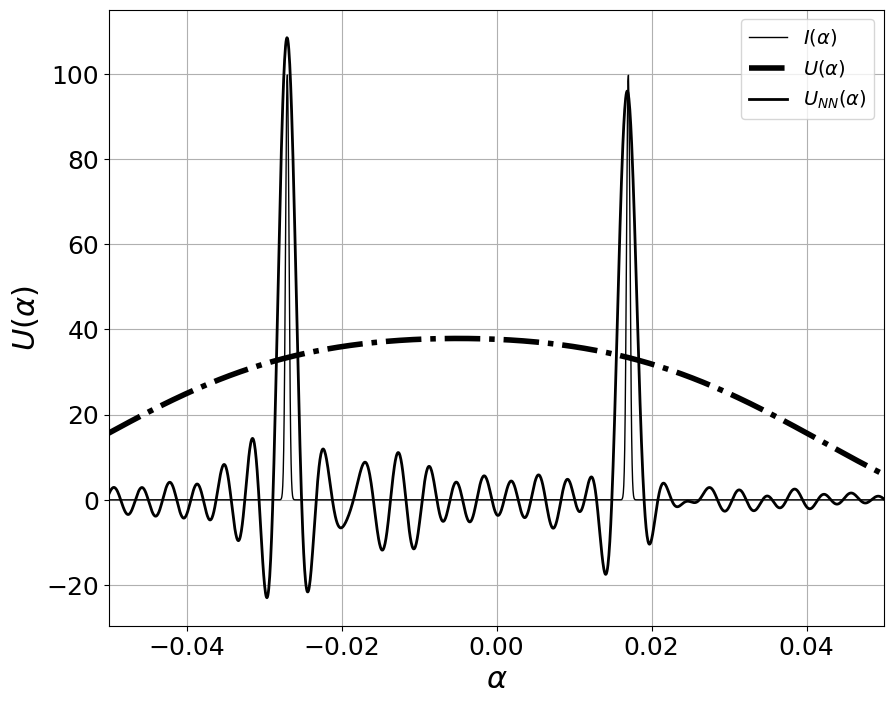
\includegraphics[width=0.65\textwidth]{Complete2_target_bw.png}
		\caption{}
		\label{fig:5}
	\end{figure}
		
	\begin{figure}[h]
		\centering
		\subfigure[]{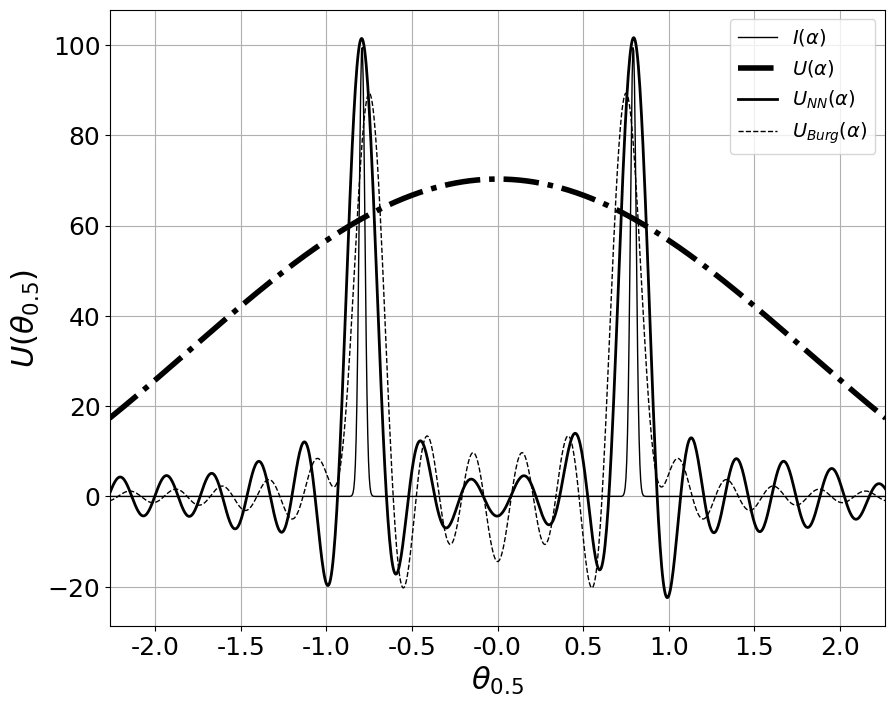
\includegraphics[width=0.45\textwidth]{Burg_NN_compare_1_bw.png}}
		\subfigure[]{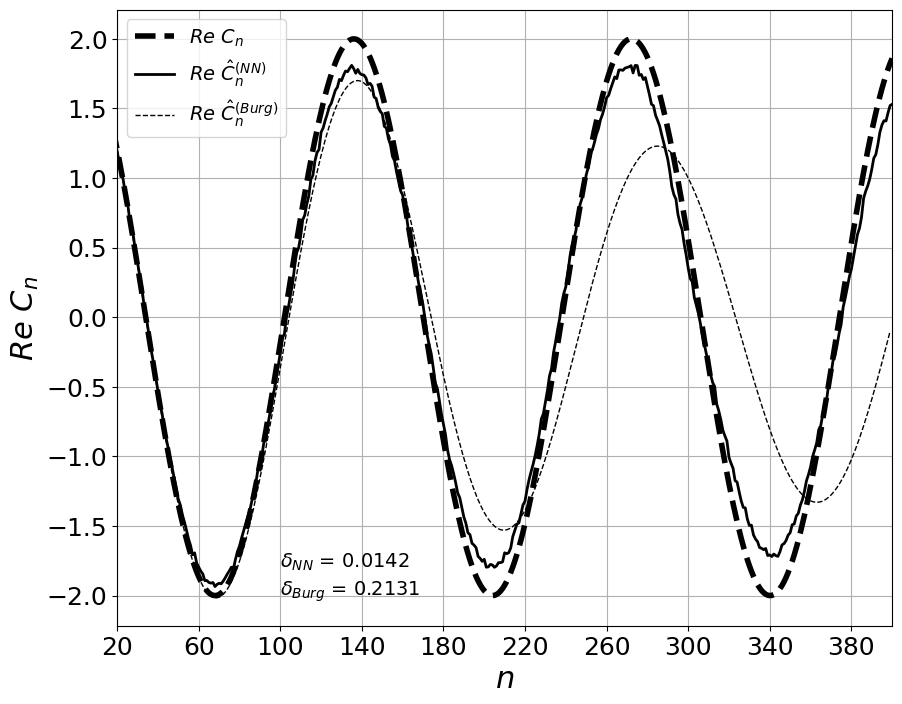
\includegraphics[width=0.45\textwidth]{Burg_NN_compare_1_real_bw.png}}
		\caption{}
		\label{fig:6}
	\end{figure}
	
	\begin{figure}[h]
		\centering
		\subfigure[]{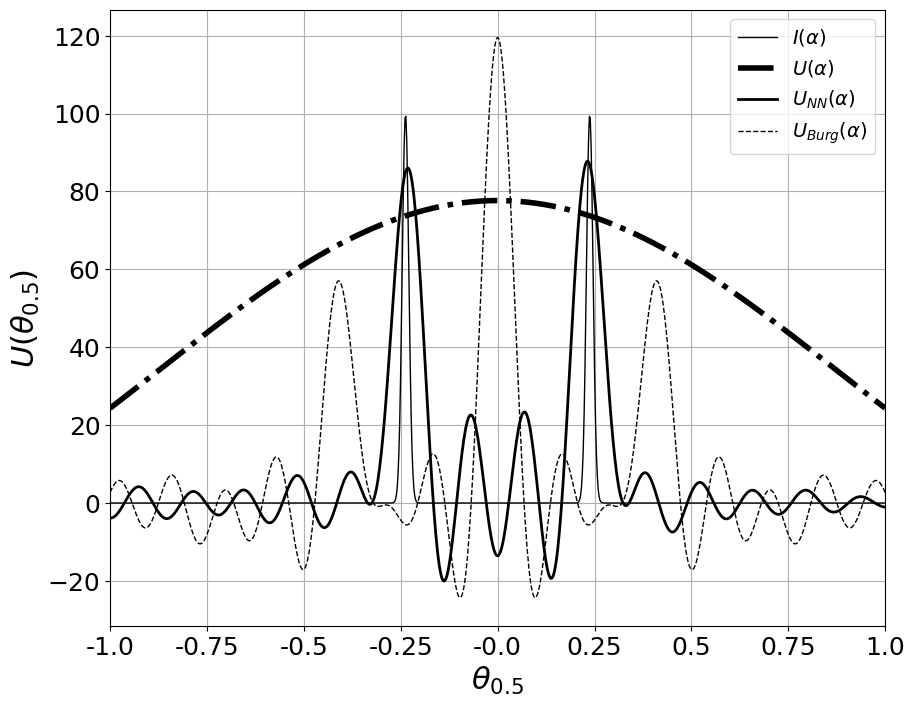
\includegraphics[width=0.45\textwidth]{Burg_NN_compare_3_bw.png}}
		\subfigure[]{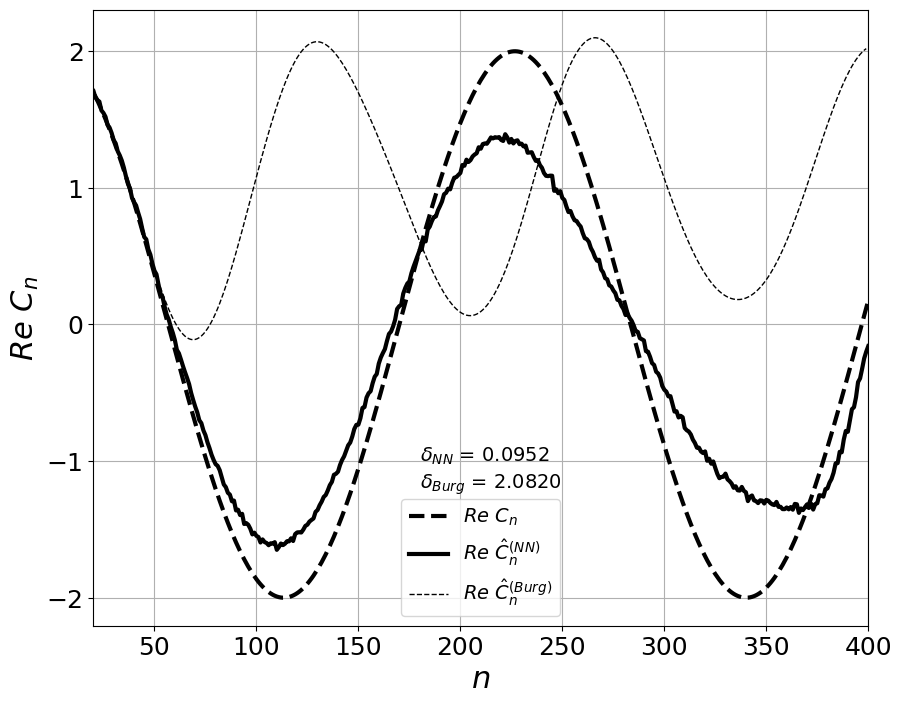
\includegraphics[width=0.45\textwidth]{Burg_NN_compare_3_real_bw.png}}
		\caption{}
		\label{fig:7}
	\end{figure}	
	
	В итоге сравним разрешающую способность, обеспечиваемую сопоставляемыми в данной работе методами экстраполяции. Для этого проведем серию экспериментов с сближающимися четными целями $t_1 = -t_2$, в которых будем измерять минимальное расстояние $theta_{p}$ при которых объекты будут все еще различимы по критерию Рэлея (\ref{raileigh}) в зависимости от числа предсказываемых значений принятого сигнала виртуальных излучателей по различным алгоритмам экстраполяции.
	
	\begin{figure}[h]
		\centering
		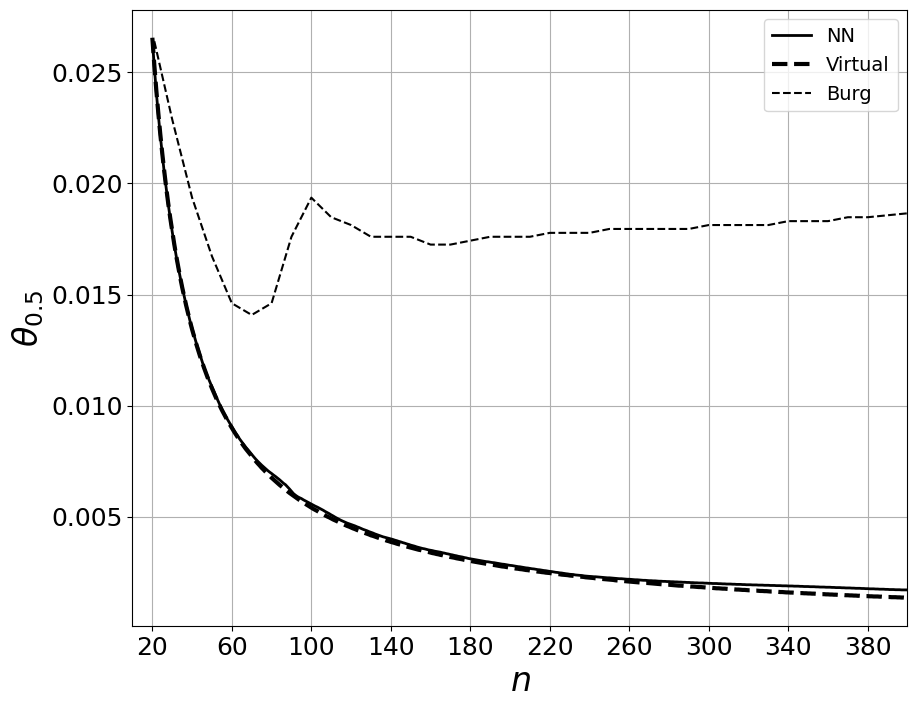
\includegraphics[width=0.65\textwidth]{berg_NN_theta_compare.png}
		\caption{График динамики показателя ширины диаграммы направленности до половинной мощности в зависимости от числа предсказываемых виртуальных устройств}
		\label{fig:8}
	\end{figure}	
	
	По построенному графику (рис. \ref{fig:8}) заметим, что добавление первых виртуальных устройств в содействие физической апертуре оказывает большее влияние на разрешающую способность по сравнению с последующими, что показывает снижающуюся эффективность добавления все более большого количества точек экстраполяции. Приблилизительное положение излучателя в заданной апертуре ЦАР, после которого ширина ДН уменьшается значительно медленнее равно $n \approx 240$. В сравнении с экстраполяцией методом нейронной сети, алгоритм экстраполяции Берга показывает худшие результаты, что обусловлено достижением плато показателя $\theta_{0.5}$ при увеличении числа точек экстраполяции. По динамике показателя также можно объяснить результаты эксперимента на рисунке (рис.\ref{fig:7}). Алгоритм Берга при увеличении виртуальной апертуры не позволяет в данной реализации экстраполяции разрешить две цели, стоящие на расстояниии $|t1 - t2| \le 0.014$. Также по графику (рис. \ref{fig:8}) можно увидеть хорошее качество работы нейронной сети для данной задачи сверхразрешения, которая проходит близко к теоретической зависимости для виртуальных устройств, работающих по модели (\ref{DN})-(\ref{coeffs_Cn}). 
	
	\section*{Заключение}
	
	
	\newpage
	
	% даём указание на включение данного место в оглавление как секции (\section)
	\addcontentsline{toc}{section}{Список используемой литературы}
	
	\begin{thebibliography}{}
		\bibitem{lit1} Bhaskar D., Rao B. D., Hari K.V.S. Performance analysis of ROOT – MUSIC // IEEE Trans. on Acoustics, Speech, and Signal Processing. 1989. Vol. ASSP – 37, pp. 1939-1949.
		
		\bibitem{lit2} Cetin M., Karl W. Feature-enhanced synthetic aperture radar image formation based on nonquadratic regularization // IEEE Trans. Image Processing. 2001. Vol. 10, №. 4, pp. 623–631.
		
		\bibitem{lit3} Quinquis A., Radoi E., Totir F. Some radar imagery results using superresolution techniques // IEEE Trans. Antennas and Propagation. 2004.Vol. 52, № 5, pp. 1230-1244, 
		
		\bibitem{lit4} Changyin S, Zheng B.  Super-resolution algorithm for instantaneous ISAR imaging // Electron. Letters. 2000. 36, № 3, pp. 253-255.
		
		\bibitem{lit5} М.В. Ратынский. Адаптация и сверхразрешение абыстродействующих антенных решетках. Радио и связ,М  2003 г. с.199.
		
		\bibitem{lit6} Herman M. A., Strohmer T. High-resolution radar via compressed sensing //  IEEE Trans. Signal Processing. 2009. Vol. 57, № 6, pp. 2275–2284.
		
		\bibitem{lit7} Lagovsky B.А. Image Restoration of the Objects with Superresolution on the Basis of Spline – Interpolation //  Progress In Electromagnetics Research Symposium (PIERS 2012-Moscow), PIERS Proceedings 2012. pp. 989 – 992.
		
		\bibitem{lit8} Лаговский Б.А., Самохин А.Б. Алгебраические методы восстановления изображения источников радиоизлучения с повышенным угловым разрешением //  Электромагнитные волны и электронные  системы.  2009, № 9, т.14,  с. 7-18.
		
		\bibitem{lit9} Лаговский Б.А. Методы повышения эффективного углового  разрешения малоразмерных целей в задачах радионавигации  и  радиолокации.  // Антенны. 2007,  № 9(124),  с. 50 -55.
		
		\bibitem{lit10} Лаговский Б.А. Восстановление изображения групповой цели цифровыми антенными решетками // Антенны. 2011. № 2(165), с. 40 -46.
		
		\bibitem{lit11} Лаговский Б.А., Рубинович Е.Я. Алгоритмы цифровой обработки данных измерений, обеспечивающие угловое сверхразрешение. Мехатроника, автоматизация, управление. 2021;22(7):349-356. https://doi.org/10.17587/mau.22.349-356
		
		\bibitem{lit12} Тормозов, В. С. Настройка, обучение и тестирование нейронной сети долгой краткосрочной памяти для задачи распознавания образов / В. С. Тормозов, А. Л. Золкин, К. А. Василенко // Промышленные АСУ и контроллеры. – 2020. – № 3. – С. 52-57. – DOI 10.25791/asu.3.2020.1171. – EDN JJWSSG.
		
		\bibitem{lit13} Минаев Е. Ю., Кутикова В. В., Никоноров А. В. Трекинг объектов в видеопотоке на основе сверточных нейронных сетей и фрактального анализа //Сборник трудов IV международной конференции и молодежной школы «Информационные технологии и нанотехнологии»(ИТНТ-2018)-Самара: Новая техника. – 2018. – С. 2792-2798.
		
		\bibitem{lit14} Козар Б. А., Кугуракова В. В., Сахибгареева Г. Ф. Структуризация сущностей естественного текста с использованием нейронных сетей для генерации трехмерных сцен //Программные продукты и системы. – 2022. – Т. 35. – №. 3. – С. 329-339.
		
		\bibitem{lit15} Семенюк В. В., Складчиков М. В. Разработка алгоритма распознавания эмоций человека с использованием сверточной нейронной сети на основе аудиоданных //Информатика. – 2022. – Т. 19. – №. 4.
		
		\bibitem{lit16} Яшин В. И. РАСТУЩИЕ НЕЙРОННЫЕ СЕТИ В РОБОТОТЕХНИКЕ //Роботизация Вооружённых Сил Российской Федерации. – 2020. – С. 279-284.
		
		\bibitem{lit17} Ахтёров А. В., Кирильченко А. А. Основы теоретической робототехники. Искусственные нейронные сети.(Обзор) //Препринты Института прикладной математики им. МВ Келдыша РАН. – 2008. – №. 0. – С. 2-20.
		
		\bibitem{lit18} Сукина С. А. Нейронные сети //Новая наука: стратегии и векторы развития. – 2016. – №. 5 (82). – С. 248.
		
		\bibitem{lit19} Ямашкин А. А., Ямашкин С. А. Использование нейронных сетей прямого распространения для ландшафтного картографирования на базе космических снимков //Геодезия и картография. – 2014. – №. 11. – С. 52-58.
		
		\bibitem{lit20} Иванько А. Ф., Иванько М. А., Сизова Ю. А. Нейронные сети: общие технологические характеристики //Научное обозрение. Технические науки. – 2019. – №. 2. – С. 17-23.
		
		\bibitem{lit21} Дычков И. Н. Сверточные нейронные сети //Тенденции развития науки и образования. – 2021. – №. 73-1. – С. 38-41.
		
		\bibitem{lit22} Назаров А.Н. Обработка потоков в мониторинговом облачном кластере. Russian Technological Journal. 2019;7(6):56-67. https://doi.org/10.32362/2500-316X-2019-7-6-56-67
		
		\bibitem{lit23} Дорожко Игорь Владимирович, Осипов Никита Алексеевич, Иванов Олег Андреевич ПРОГНОЗИРОВАНИЕ ТЕХНИЧЕСКОГО СОСТОЯНИЯ СЛОЖНЫХ ТЕХНИЧЕСКИХ СИСТЕМ С ПОМОЩЬЮ МЕТОДА БЕРГА И БАЙЕСОВСКИХ СЕТЕЙ // Труды МАИ. 2020. №113.
		
		\bibitem{lit24} Виноградова Е. П., Головин Е. Н. Метрики качества алгоритмов машинного обучения в задачах классификации //Научная сессия ГУАП. – 2017. – С. 202-206.
		
		\bibitem{lit25} Шишкин Ю. Е., Скатков А. В. Метрики качества для оценки и прогнозирования критических состояний //Качество и жизнь. – 2019. – №. 1. – С. 61-66.
		
		\bibitem{lit26} Каширина И. Л., Демченко М. В. Исследование и сравнительный анализ методов оптимизации, используемых при обучении нейронных сетей //Вестник ВГУ. Серия: Системный анализ и информационные технологии. – 2018. – №. 4. – С. 123-132.
	\end{thebibliography}
	
\end{document}